% !TEX root = INT.tex

\chapter{Signal Region Definition}
\label{chap:SignalRegion}

\section{Physical Intuition on how Signal Region Selections Reject SM Background}
\label{sec:SR:Selections}

\indent The kinematic selection in the signal region is designed to reject SM ttbar events while retaining signal.  After the zero lepton preselection, single hadronic tau and single lepton ttbar makes up 95 percent of the ttbar background because fully hadronic ttbar generates no neutrinos and therefore $\MET$.   Because we select for events with least $250 \gev$ of $\MET$, the top that decays leptonically must be boosted.  The leptonic top can gain boost by recoiling against the other hadronic top in a back to back fashion.  Alternatively both tops can be boosted by strong initial state radiation.   A detailed description of the $\ttbar$ background and these two distinct populations is given in section \ref{sec:Bkg:ttbar}.  \\

\indent 90 percent of all ttbar events after pre-selection belong to the two tops back to back population.  It is simply easier to boost one top against the other instead of having to both tops with additional strong initial state radiation.  At the same time, the kinematics of the two tops back to back ttbar population is very different from those of the signal.  This means we are able to reject the majority of the two tops back to back population without loosing too much signal. \\

\begin{figure}[h!]
  \centering
	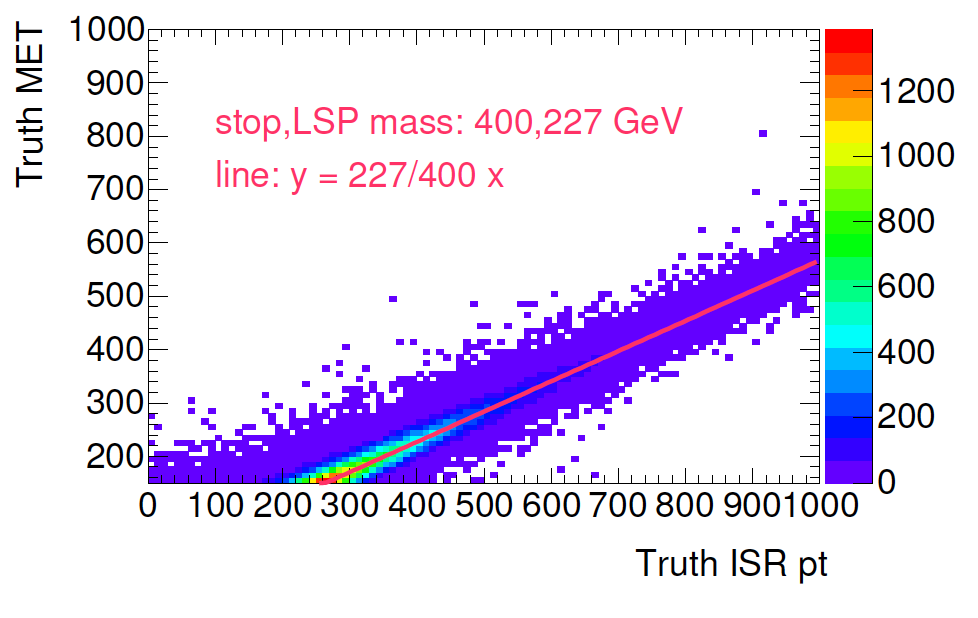
\includegraphics[width=0.65\textwidth]{./figures/MET_ISR.png}
\caption{\label{fig:ttbar:3pop}{Basic depiction of the kinematics of the two ttbar populations and stop plus strong ISR events after 0 lepton pre-selection }}
\end{figure}

\indent Figure \ref{fig:ttbar:3pop} shows examples of the three different populations lined up along their thrust axis with the hemisphere containing the \MET in the upper half.  The hemisphere with the \MET contains significantly more jets and a total higher energy in signal then the ttbar two tops back to back population.  The signal has 6 jets originating from the two hadronic tops in the hemisphere with \MET instead of only a single leptonic top in the ttbar back to back population.   The ttbar with strong ISR population looks more signal like as it has higher jet multiplicity and energy in the \MET hemisphere however, it still has less total energy then that of signal. \\

\indent By cutting on the jet multiplicity and total energy in the hemisphere with \MET we are able to reject 98 to 99 percent of ttbar events which already passed preselection but have less then 400 GeV of true ISR pt.  Acceptance of ttbar events increase with high ISR pt but only asymptotically.  Even at 1200 GeV of true ISR pt, a ttbar event which already passed zero lepton preselection only has a 35 percent chance of passing the additional signal region selection.  \\

\indent After 0 lepton preselection, the signal to background ratio is 1 to 40 for a stop mass of 400 GeV.  After signal region selection we get an around 2 to 1 signal to background ratio for the same mass point.  This resounding success in eliminating background can largely be attributed to the signal region selection's efficiency in eliminating the dominant back to back ttbar population and significantly reducing the lesser ttbar plus strong ISR population all the while retaining most of signal. \\

\indent At the same time, the same kinematic selections on jet multiplicity and total energy is also difficult for sub-dominant backgrounds such as $W$+jets, $Z$+jets, single top and QCD multijet to satisfy.  In general it is difficult for these other processes to produce such high jet multiplicity and total energy in the same half of the event as the $\MET$.   Processes such as $W$+jets and $Z$+jets normally have the $\MET$ recoiling against other energetic jets.  Therefore, most energetic jets in these processes tend to lie in the hemisphere opposite the $\MET$.  After signal selection, the dominate background is still standard model ttbar which comprises over 90 percent of all backgrounds in the SR.

\section{Kinematic Variables Definitions}
\label{sec:SR:Definitions}

The kinematic variables used are reconstructed using the recursive jigsaw method.  A detailed description of this method and variable defined can be found in section \ref{Jigsaw:ISR}.  In short, the recursive jigsaw method separates the event into two hemispheres according to the thrust axis.  The thrust axis is the axis that maximizes the amount of back to back momenta along it and should approximate the direction of initial state radiation and sparticle back to back recoil in events with strong ISR.  The hemisphere containing the $\MET$ is considered the "sparticle" hemisphere and the hemisphere opposite the $\MET$ is considered the ISR hemisphere.  All jets in the sparticle hemisphere is considered to have originated from one of the stop decays.  All jets in the ISR hemisphere is considered to be an ISR jet.  The performance of this ISR identification algorithm can be found in section \ref{Jigsaw:Performance}. \\
We construct variables that measure kinematic properties of both the ISR and sparticle hemispheres.  Those variables are listed below: \\

\begin{description}
\item [\boldmath \nBJetS:] number of b-tagged jets associated with the sparticle hemisphere.
\item [\boldmath \nJetS:] number of jets associated with the sparticle hemisphere.
\item [\boldmath \pTSBZero:] \pt\ of the leading b-jet in the sparticle hemisphere.
\item [\boldmath \pTSFour:] \pt\ of the fourth jet ordered in \pt\ in the sparticle hemisphere.
\item [\boldmath \dPhiISRMET:] angular separation in $\phi$ of the ISR and the \met in the CM frame.
\item [\boldmath \pTISR:] \pt\ of the ISR system, evaluated in the CM frame.
\item [\boldmath \mS:] transverse mass between the whole sparticle system and \met.
\item [\boldmath \mV/\mS:] ratio of the transverse mass of the only the visible part of the sparticle system without \met and the whole sparticle system including \met.
\item [\boldmath \rISR:] Ratio between invisible system (\met in CM frame) and \pTISR
\end{description}

$\NbV$ and $\NjV$ describes the jet multiplicity of the sparticle system.  $\MS$, $\pTjV$, and $\pTSBZero$ are all related to the total energy in the sparticle system.  $\pTISR$ corresponds to the total $\pt$ of the ISR system.  Finally $\RISR$ and $\dphiISRI$ describe the correlation between the ISR system and $\MET$ in both direction and magnitude. \\

\section{Signal Region Kinematic Selection}
\label{sec:SR:Selections}

Kinematic Selections for Signal Region is defined in table \ref{tab:SignalRegionC}.\\

\begin{table}[htpb]
  \caption{Signal region definitions, in addition to the preselection requirements presented in Table~\ref{tab:SRcommon}. }
  \begin{center}
    \def\arraystretch{1.4}%
    \begin{tabular}{c||c|c|c|c|c|} \hline\hline
      {\bf Variable} & SRC-1 & SRC-2 & SRC-3 & SRC-4 & SRC-5 \\ \hline \hline
       b-tagged jets & \multicolumn{5}{c}{$\ge1$} \\ 
      \nBJetS & \multicolumn{5}{c}{$\ge1$} \\
      \nJetS & \multicolumn{5}{c}{$\ge5$}  \\
      \pTISR & \multicolumn{5}{c}{$>400$ GeV}   \\ \hline
      \pTSBZero & \multicolumn{5}{c}{$>40\gev$}  \\ 
      \pTSFour & \multicolumn{5}{c}{$>50$ GeV}   \\ 
      \mS & \multicolumn{5}{c}{$>300\gev$}  \\ \hline
      \dPhiISRMET & \multicolumn{5}{c}{$>3.00$}  \\ 
      \rISR &  0.30-0.40 & 0.40-0.50 & 0.50-0.60 & 0.60-0.70 & 0.70-0.80\\  \hline \hline
    \end{tabular}
  \end{center}
  \label{tab:SignalRegionC}
\end{table}%

\indent The selections on $\nJetS$ and $\nBJetS$ ensures that the hemisphere with $\MET$ has high amounts of jet multiplicity.  This requirement is naturally satisfied in signal events because the two neutralinos naturally go in the same direction as the six jets resulting from the two stop decays.  However this requirement is difficult for the two top back to back population to satisfy since only a single leptonic or hadronic tau top is in the same hemisphere as the $\MET$ in the hard process.  \\

\indent The ttbar plus strong ISR population is able to pass this selection as both the leptonic and hadronic tops are in sparticle hemisphere in this case.  The result is the main background is ttbar plus strong ISR pt events pass after a requirement on the sparticle jet multiplicity and the $\pTISR > 400 \GeV$ requirement.  Signal to background ratio is around 1 to 5 after these selections.  {\bf NEEDS PLOTS}\\

\indent Distribution of different kinematic variables is shown after a requirement on $\pTISR$, $\nJetS$, and $\nBJetS$ is shown in figure \ref{fig:SR:jetMultiplicity}. The ttbar MC is normalized to a 1 lepton control region with the same selections on sparticle jet multiplicity, and $\pTISR$.  All sub-dominant background are normalized to their respective CRs defined in section \ref{sec:Bkg:sub}.\\

\begin{figure}[htbp]
  \begin{center}
    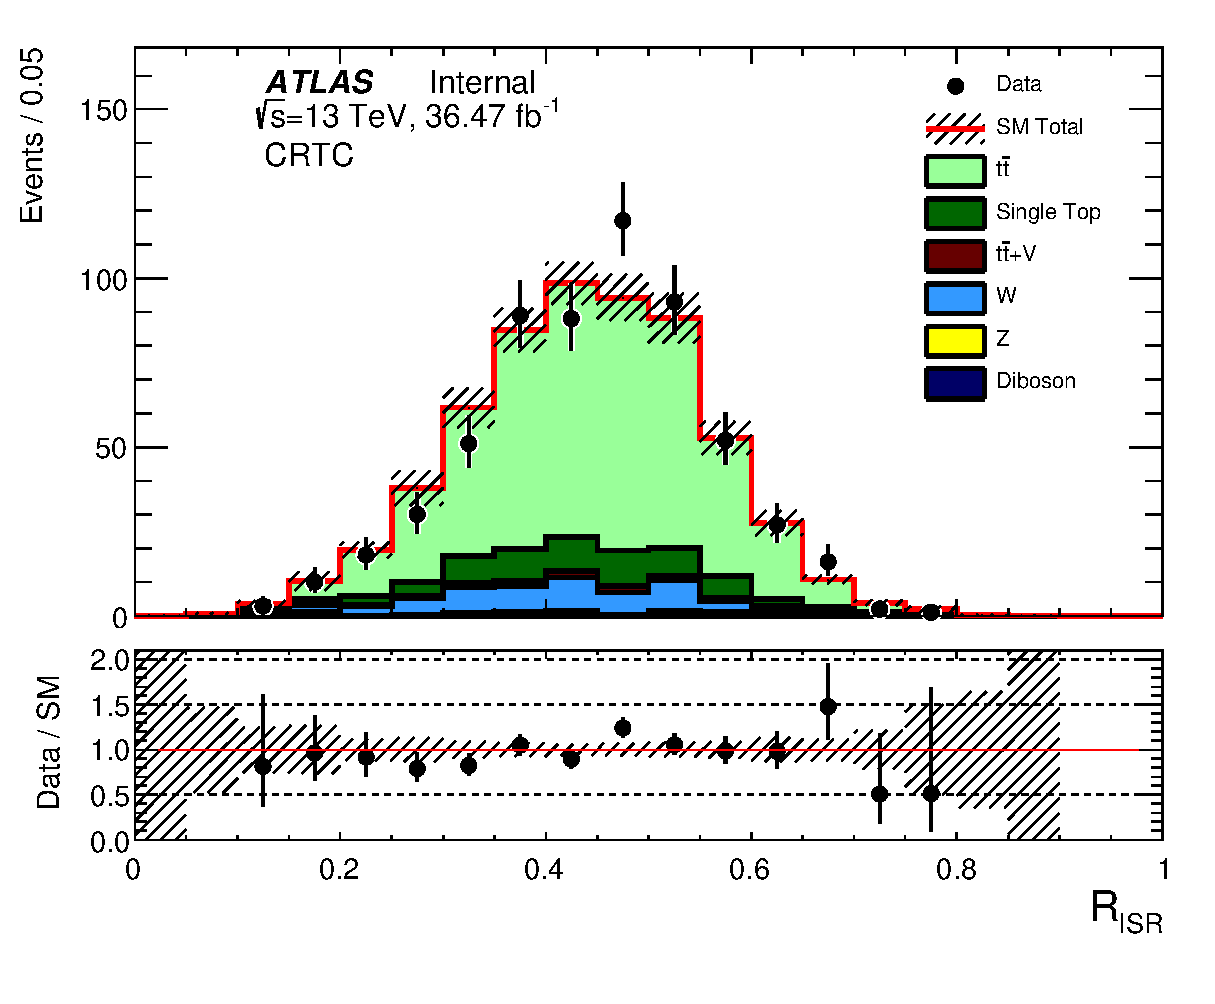
\includegraphics[width=0.45\textwidth]{figures/ttbar/postfit/CA_RISR_CRTopC}
    \includegraphics[width=0.45\textwidth]{figures/ttbar/postfit/CA_pTISR_CRTopC}
    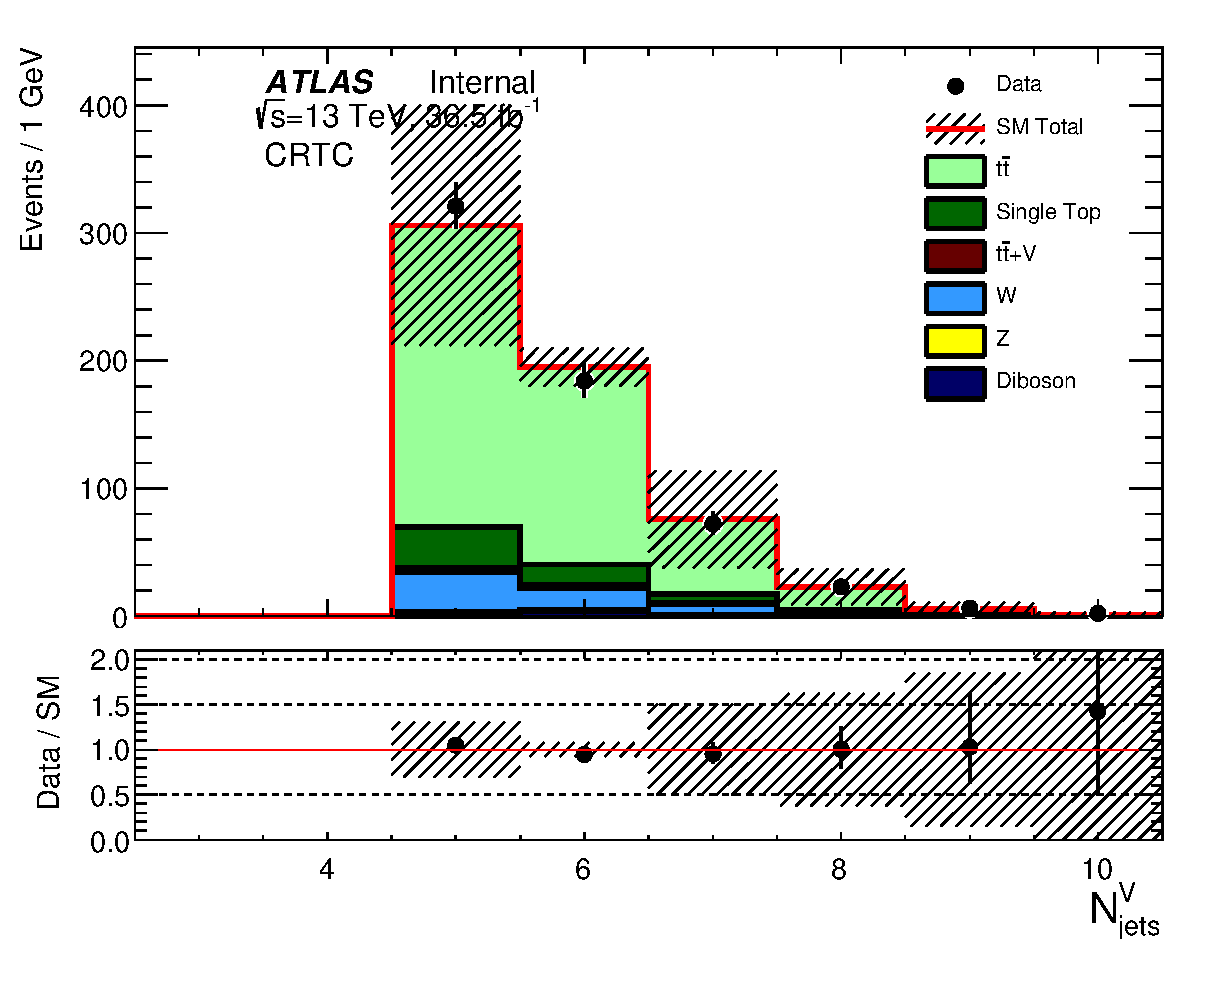
\includegraphics[width=0.45\textwidth]{figures/ttbar/postfit/CA_NjV_CRTopC}
    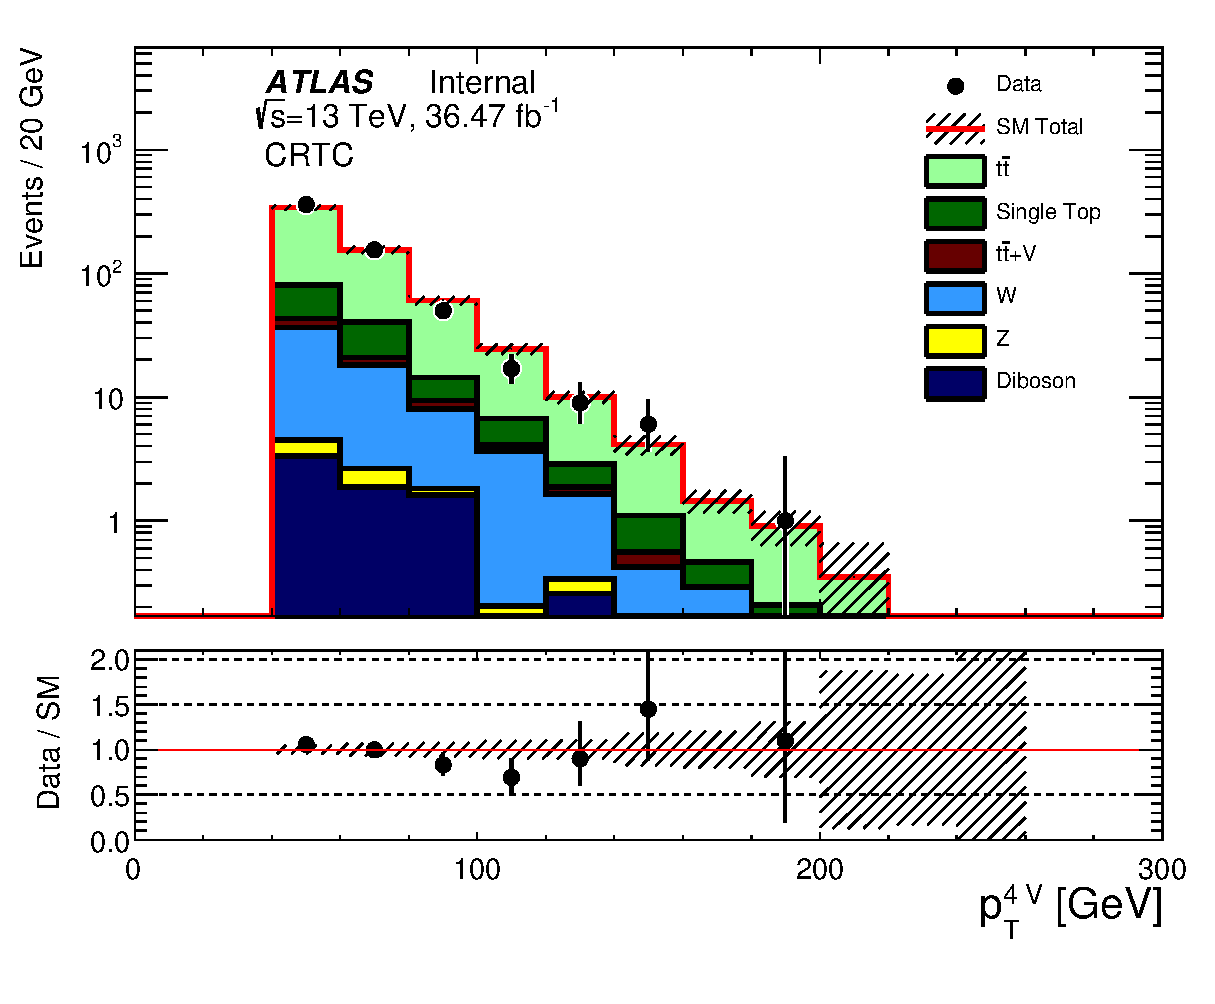
\includegraphics[width=0.45\textwidth]{figures/ttbar/postfit/CA_pTjV4_CRTopC_log}
    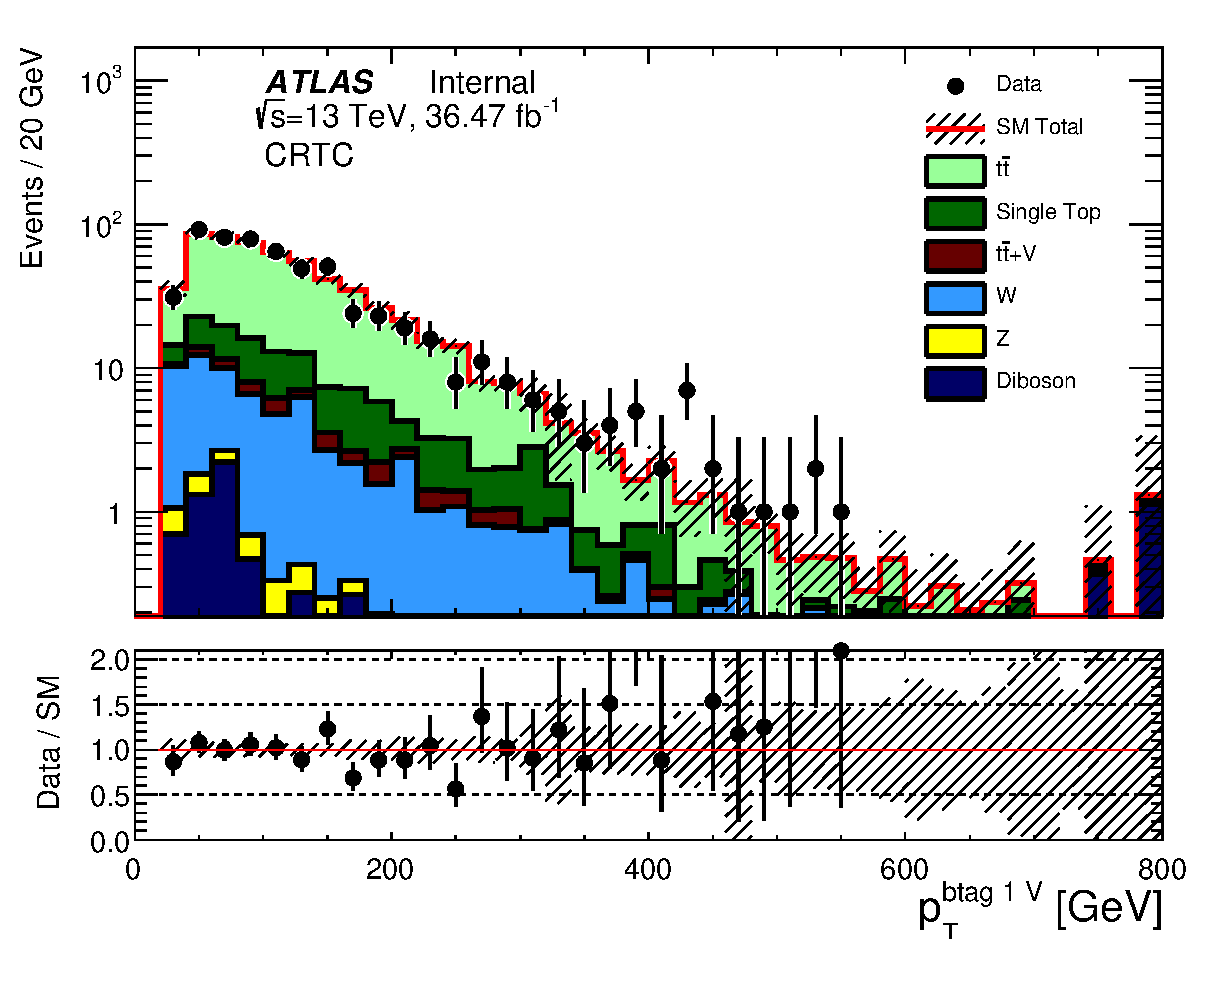
\includegraphics[width=0.45\textwidth]{figures/ttbar/postfit/CA_pTbV1_CRTopC_log}
        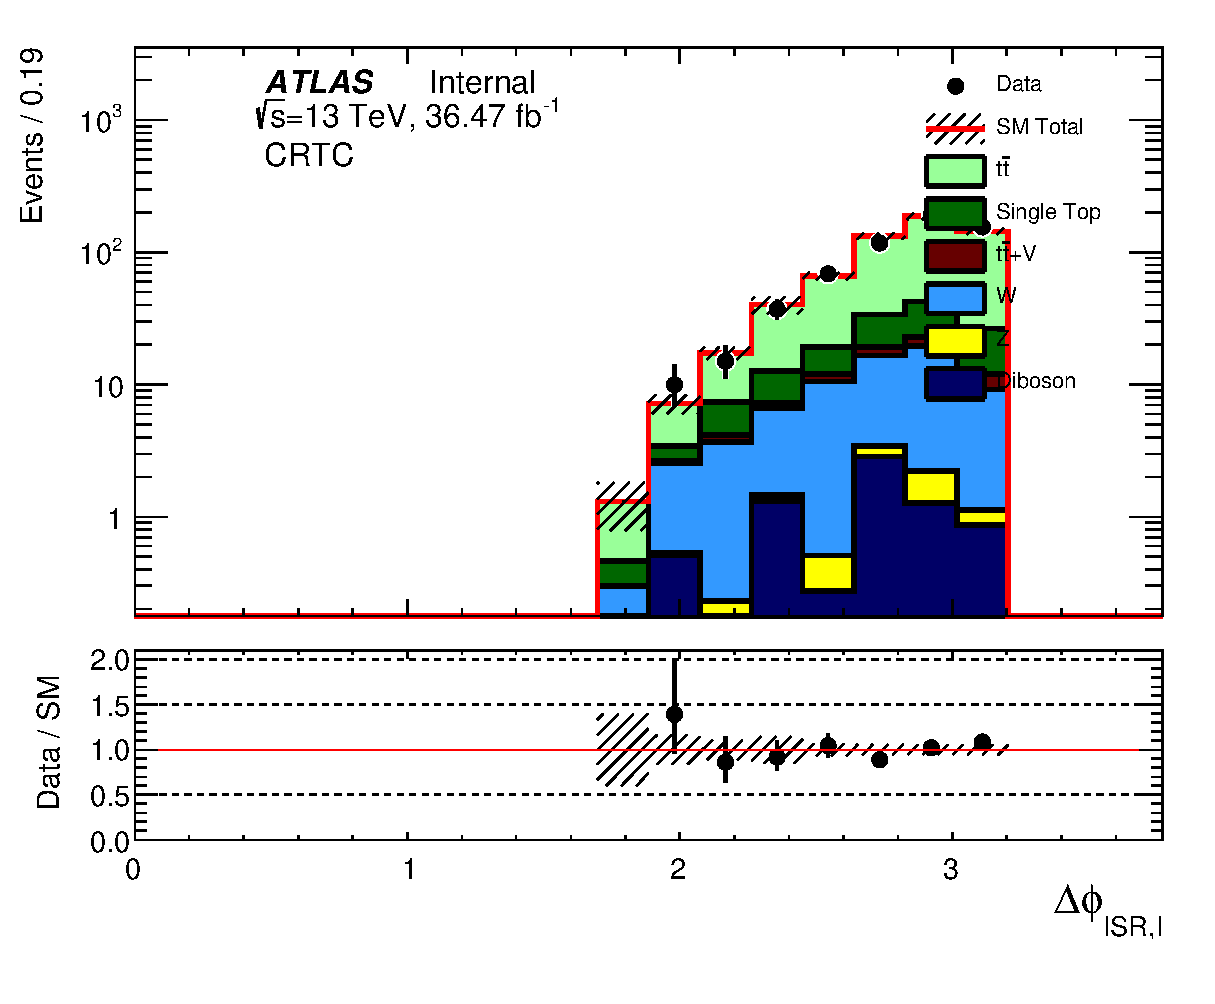
\includegraphics[width=0.45\textwidth]{figures/ttbar/postfit/CA_dphiISRI_CRTopC_log}
  \end{center}
  \caption{{\bf NEEDS PLOTS} Distributions for 0 lepton preselection plus $\pTISR > 400 \gev$, $\nBJetS\ge1$  and $\nJetS\ge5$ with \intlumi\ \ifb\ of data. The ratio between data and MC is shown in the bottom panel. The hashed area in both the top and lower panel represent the uncertainty due to MC statistics and detector plus theoretical systematic uncertainties}
  \label{fig:SR:jetMultiplicity}
\end{figure}

\indent Next we make a requirement on the total energy of the sparticle system.  The total transverse mass of the sparticle system $\mS$ must be greater then $300 \gev$ and the $\pt$ of the jet with 4th highest $\pt$ in the sparticle system must be greater then $50 \gev$.  $\pTSBZero$ must also be greater then $40 \gev$.   \\

\indent In general, the signal with two fully hadronic tops has more energy in the sparticle hemisphere then ttbar.  The two top back to back recoil population is nearly eliminated by these selections.  Of the ttbar events that passed 0 lepton preselection, less then 2 percent of ttbar events with true ISR pt less then $400 \gev$ pass these selections.  Even for ttbar events with greater then $600 \gev$ of true ISR pt, the selection is difficult to satisfy.  Only 35 percent of the ttbar with greater then 600 GeV and also passed the 0 lepton preselection pass the addition requirement on sparticle jet multiplicity and energy.  Signal to background ratio improves to around 1 to 2 after these selections. \\

\indent Distribution of various kinematic variables after sparticle jet multiplicity, $\pTISR$, and sparticle energy requirement is shown in figure \ref{fig:SR:sparticleEnergy}.  The ttbar MC is normalized to a 1 lepton control region with the same selections on sparticle jet multiplicity, $\pTISR$, and sparticle energy requirement.  All sub-dominant background are normalized to their respective CRs defined in section \ref{sec:Bkg:sub}.\\
\begin{figure}[htbp]
  \begin{center}
    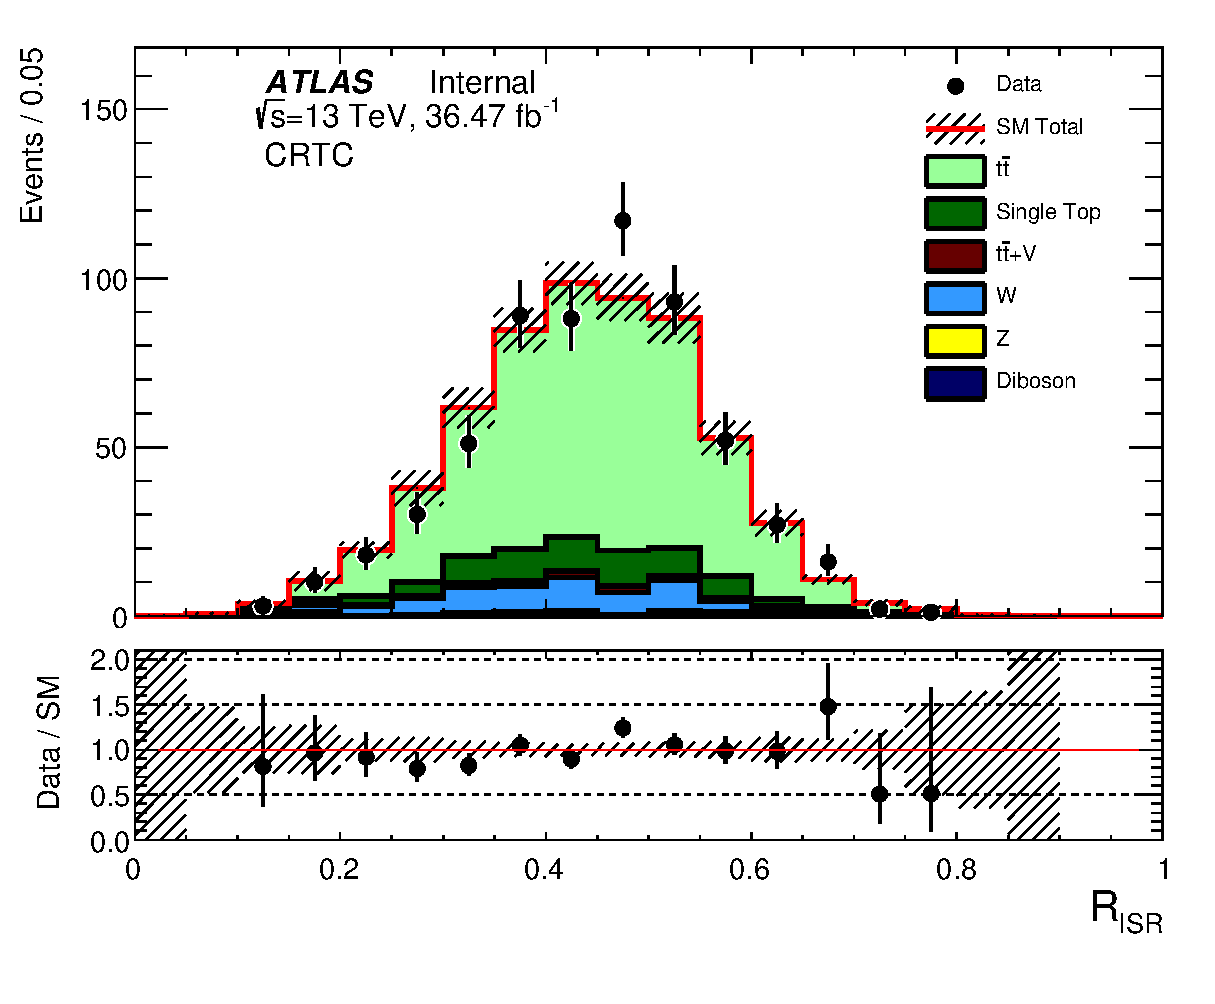
\includegraphics[width=0.45\textwidth]{figures/ttbar/postfit/CA_RISR_CRTopC}
    \includegraphics[width=0.45\textwidth]{figures/ttbar/postfit/CA_pTISR_CRTopC}
    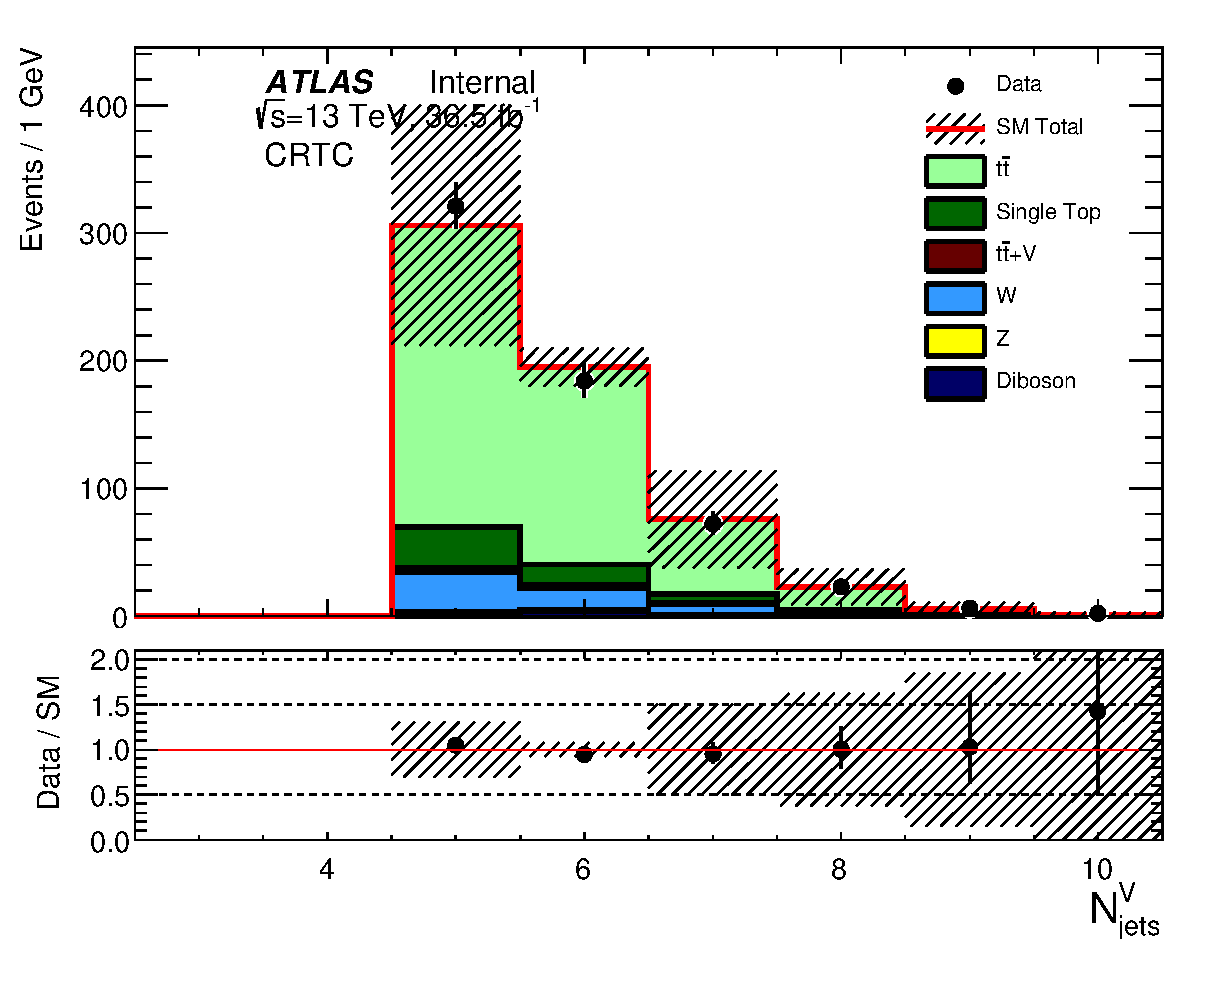
\includegraphics[width=0.45\textwidth]{figures/ttbar/postfit/CA_NjV_CRTopC}
    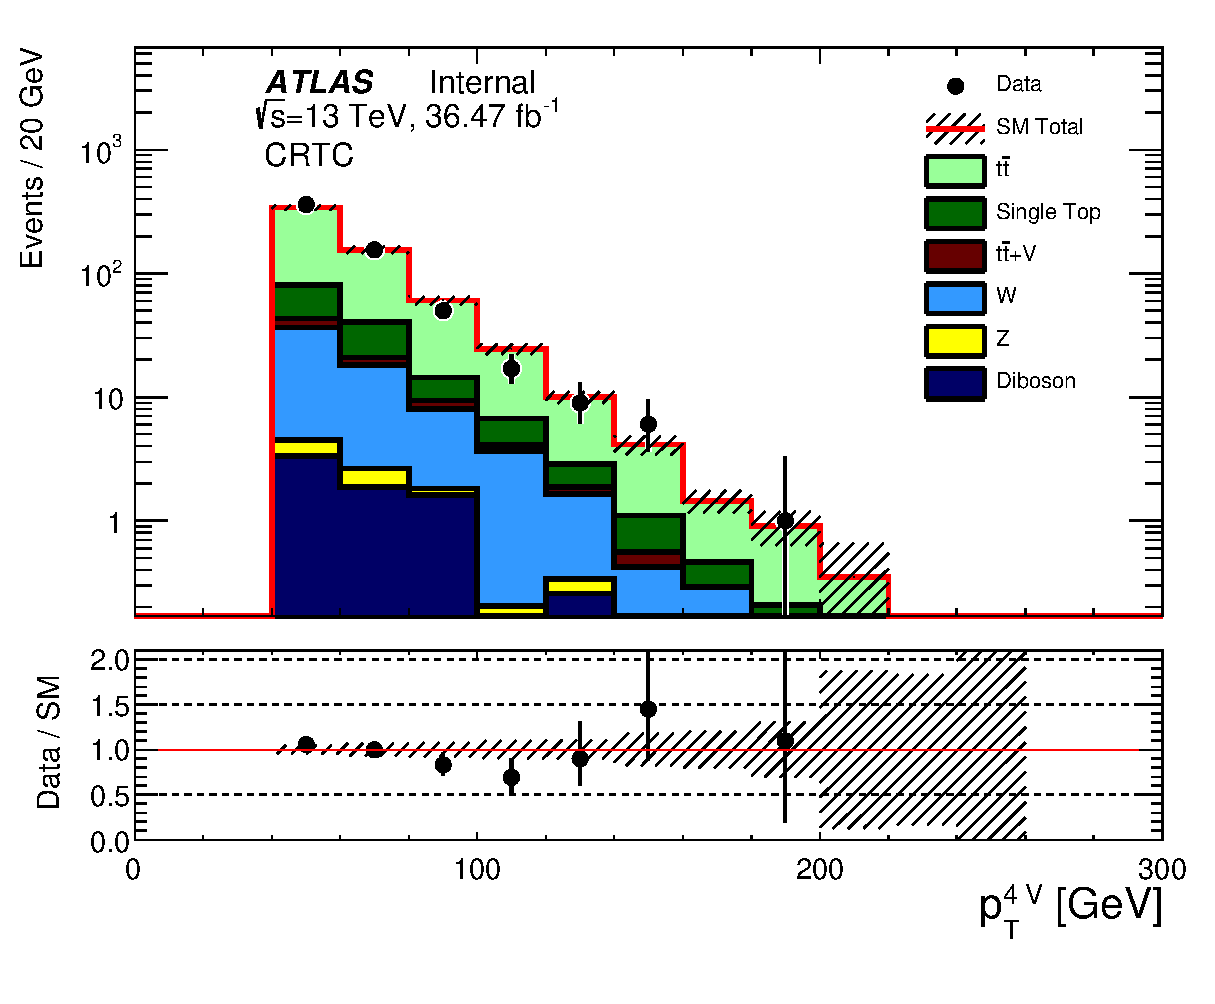
\includegraphics[width=0.45\textwidth]{figures/ttbar/postfit/CA_pTjV4_CRTopC_log}
    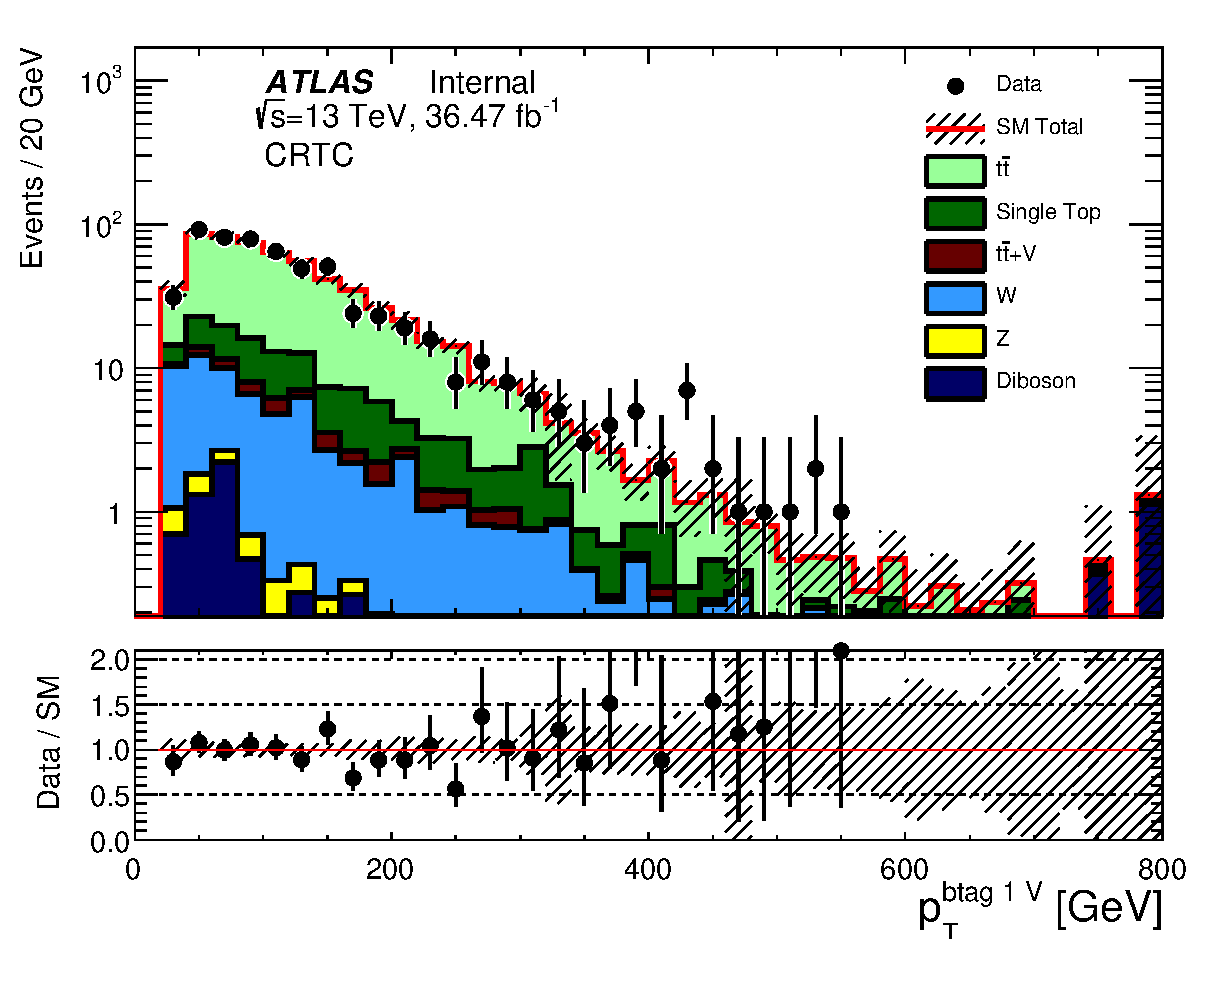
\includegraphics[width=0.45\textwidth]{figures/ttbar/postfit/CA_pTbV1_CRTopC_log}
  \end{center}
  \caption{{\bf NEEDS PLOTS} Distributions for 0 lepton preselection plus sparticle jet multiplicity, $\pTISR$, and sparticle total energy requirement with \intlumi\ \ifb\ of data. The ratio between data and MC is shown in the bottom panel. The hashed area in both the top and lower panel represent the uncertainty due to MC statistics and detector plus theoretical systematic uncertainties}
  \label{fig:SR:sparticleEnergy}
\end{figure}

\indent Lastly we make the a selections on correlations between the $\MET$ and ISR systems.  $\dPhiISRMET > 3.0$ ensures the $\MET$ and ISR systems are back to back.  The ISR system and $\MET$ must be nearly back to back in signal because the neutralino gains momenta mainly from ISR.  SM ttbar on the other hand do not need to have back to back $\MET$ and ISR systems.  Although the $\MET$ and ISR are also correlated for SM ttbar, the neutrino from the single lepton top decay gain some momenta from the top decay itself and can go in a different direction. The same logic holds for subdominant backgrounds such as $W$+jet and single top. \\

\indent The distribution of $\dPhiISRMET$ with all previous selections on sparticle jet multiplicity and sparticle system energy applied is shown in figure \ref{fig:SR:dphiISRMET}.   The ttbar MC is normalized to a 1 lepton control region with the same selections on sparticle jet multiplicity, $\pTISR$, and sparticle energy requirement.  All sub-dominant background are normalized to their respective CRs defined in section \ref{sec:Bkg:sub}. \\

\begin{figure}[htbp]
  \begin{center}
     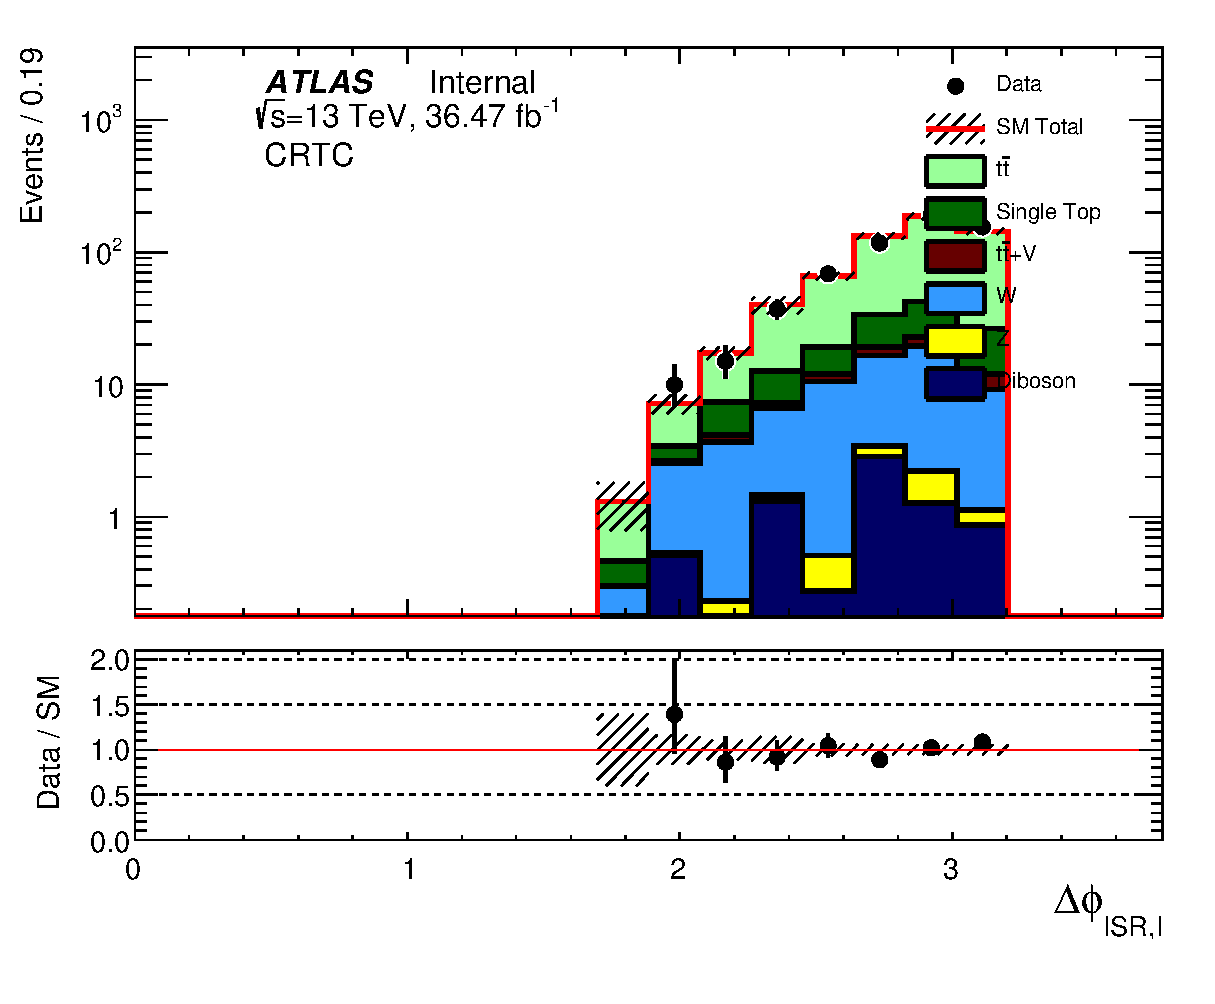
\includegraphics[width=0.45\textwidth]{figures/ttbar/postfit/CA_dphiISRI_CRTopC_log}
  \end{center}
  \caption{{\bf NEEDS PLOTS} $\dPhiISRMET$ distributions for 0 lepton preselection plus sparticle jet multiplicity, $\pTISR$, and sparticle total energy requirement with \intlumi\ \ifb\ of data. The ratio between data and MC is shown in the bottom panel. The hashed area in both the top and lower panel represent the uncertainty due to MC statistics and detector plus theoretical systematic uncertainties}
  \label{fig:SR:dphiISRMET}
\end{figure}

\indent After we get the final $\RISR$ distribution shown in figure \ref{fig:SR:RISR}. The ttbar MC is normalized to a 1 lepton control region defined in table \ref{tab:ttbar1LepCRISR_def}.  All sub-dominant background are normalized to their respective CRs defined in section \ref{sec:Bkg:sub}.\\

\begin{figure}[htbp]
  \begin{center}
     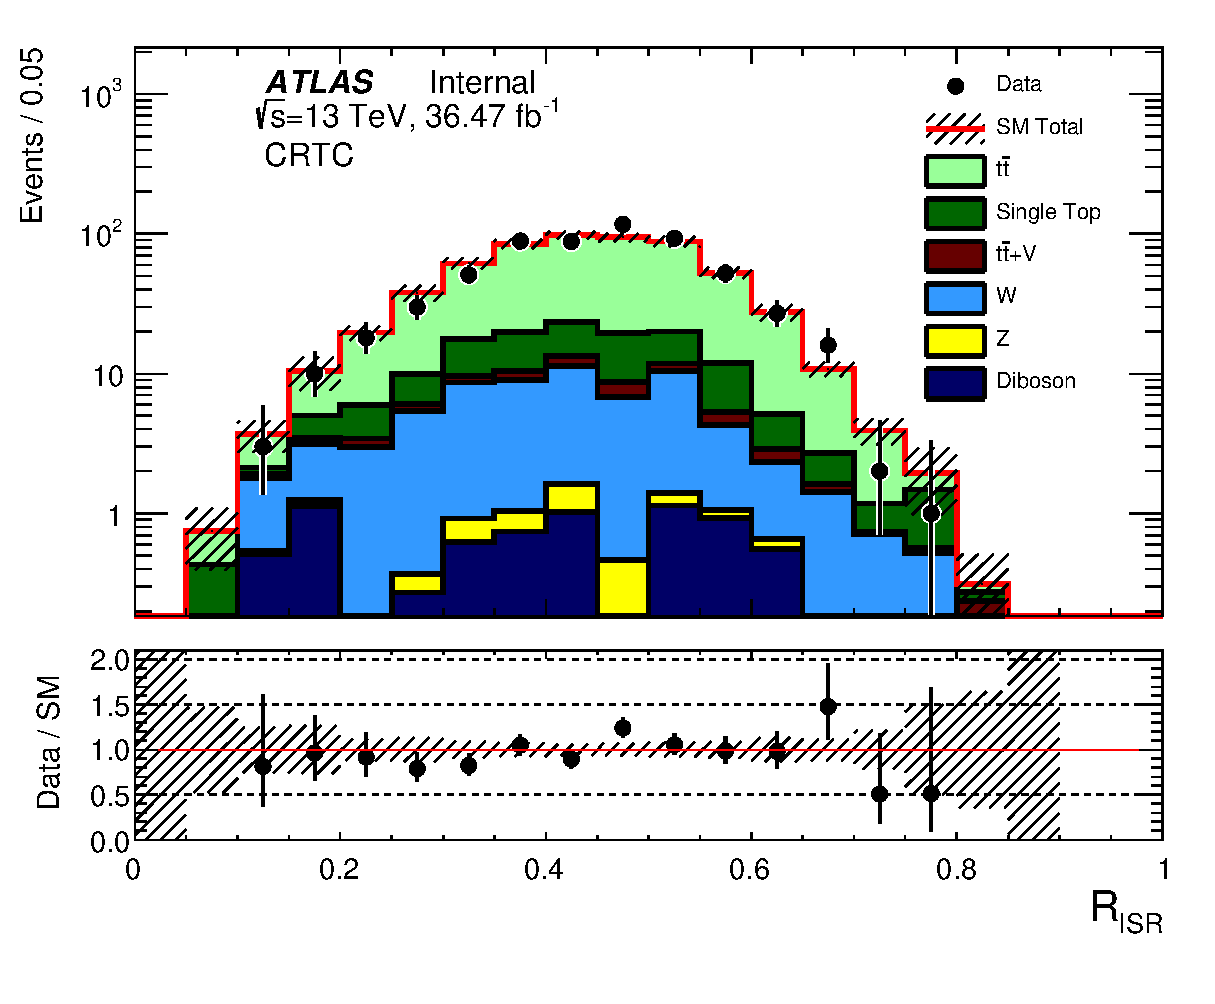
\includegraphics[width=0.45\textwidth]{figures/ttbar/postfit/CA_RISR_CRTopC_log}
  \end{center}
  \caption{{\bf NEEDS PLOTS} $\RISR$ distribution after signal region selection with \intlumi\ \ifb\ of data. The ratio between data and MC is shown in the bottom panel. The hashed area in both the top and lower panel represent the uncertainty due to MC statistics and detector plus theoretical systematic uncertainties}
  \label{fig:SR:RISR}
\end{figure}

\indent This $\RISR$ distribution is then separated into $5$ bins from $0.3$ to $0.8$.  We expect to receive very little signal events in $\RISR$ below 0.3.  At the same time, the region of $\RISR$ below 0.3 is dominated by QCD background and serves as a validation region for QCD multijet background.  \\

\indent Stop samples with different stop and neutralino masses will peak in different locations in $\RISR$ with a signal to background ratio of about 2 to 1 under the peak.  The simultaneous fit to all five bins captures the feature of the signal peak in $\RISR$.  \\

\section{Signal Region Expected Yields and Kinematic Distributions}
\label{sec:SR:Yields}

\indent The expected yields in the signal region is given in table \ref{tab:SRyield}.  All backgrounds have been normalized to control regions defined in chapter \ref{chap:backgrounds}.  Signal yields for three example signal samples with stop, neutralino masses of $(300,127 \gev), (400,227\gev), $ and $(500,327 \gev)$ are also shown for comparison.  In general between 1 to 1 or 2 to 1 signal to background ratio is achieved in the signal peak in RISR. \\

\begin{table}
  \begin{center}
    \def\arraystretch{1.4}%
    \begin{tabular}{c|c}
\hline\hline
\multicolumn{2}{c}{\bf SRC1 } \\ \hline 
Z & 0.11 $\pm$ 0.03 \\
dibosons & 0.04 $\pm$ 0.04 \\
ttbar & 1.99 $\pm$ 0.46 \\
singleTop & 0.09 $\pm$ 0.06 \\
ttV & 0.03 $\pm$ 0.04 \\
W & 0.46 $\pm$ 0.23 \\
\hline
Total MC & 2.72 $\pm$ 0.52 \\
\hline\hline
\end{tabular}

    \begin{tabular}{c|c}
\hline\hline
\multicolumn{2}{c}{\bf SRC2 } \\ \hline 
Z & 0.90 $\pm$ 0.13 \\
dibosons & 0.21 $\pm$ 0.21 \\
ttbar & 31.20 $\pm$ 1.82 \\
singleTop & 1.02 $\pm$ 0.19 \\
ttV & 0.46 $\pm$ 0.19 \\
W & 1.53 $\pm$ 0.31 \\
\hline
Total MC & 35.30 $\pm$ 1.88 \\
Data & 22.00 $\pm$ 4.69 \\
\hline
(500,327) GeV & 1.42 $\pm$ 0.26  \\
\hline
(300,127) GeV & 72.20 $\pm$ 7.29  \\
\hline
(400,227) GeV & 10.81 $\pm$ 1.00 \\
\hline\hline
\end{tabular}

    \begin{tabular}{c|c}
\hline\hline
\multicolumn{2}{c}{\bf SRC3 } \\ \hline 
Z & 0.74 $\pm$ 0.15 \\
dibosons & 0.28 $\pm$ 0.28 \\
ttbar & 20.62 $\pm$ 1.07 \\
singleTop & 1.04 $\pm$ 0.41 \\
ttV & 0.44 $\pm$ 0.11 \\
W & 1.51 $\pm$ 0.37 \\
\hline
Total MC & 24.64 $\pm$ 1.25 \\
Data & 22.00 $\pm$ 4.69 \\
\hline
 ($\mstop$, $\mLSP$) = (500,327) GeV & 6.90 $\pm$ 0.56 (1.3$\sigma$) \\
\hline
 ($\mstop$, $\mLSP$) = (300,127) GeV & 14.80 $\pm$ 2.56 (2.7$\sigma$) \\
\hline
 ($\mstop$, $\mLSP$) = (400,227) GeV & 30.01 $\pm$ 1.67 (5.2$\sigma$) \\
\hline\hline
\end{tabular}

    \begin{tabular}{c|c}
\hline\hline
\multicolumn{2}{c}{\bf SRC4 } \\ \hline 
Z & 0.45 $\pm$ 0.09 \\
dibosons & 0.00 $\pm$ 0.00 \\
ttbar & 6.95 $\pm$ 0.46 \\
singleTop & 0.62 $\pm$ 0.17 \\
ttV & 0.07 $\pm$ 0.08 \\
W & 1.53 $\pm$ 0.41 \\
\hline
Total MC & 9.61 $\pm$ 0.65 \\
Data & 1.00 $\pm$ 1.00 \\
\hline
 ($\mstop$, $\mLSP$) = (500,327) GeV & 10.53 $\pm$ 0.68 (2.9$\sigma$) \\
\hline
 ($\mstop$, $\mLSP$) = (300,127) GeV & 0.80 $\pm$ 0.57 (0.1$\sigma$) \\
\hline
 ($\mstop$, $\mLSP$) = (400,227) GeV & 8.95 $\pm$ 0.86 (2.5$\sigma$) \\
\hline\hline
\end{tabular}

    \begin{tabular}{c|c}
\hline\hline
\multicolumn{2}{c}{\bf SRC5 } \\ \hline 
Z & 0.44 $\pm$ 0.10 \\
dibosons & 0.15 $\pm$ 0.10 \\
ttbar & 6.33 $\pm$ 0.72 \\
singleTop & 0.53 $\pm$ 0.14 \\
ttV & 0.08 $\pm$ 0.08 \\
W & 1.38 $\pm$ 0.37 \\
\hline
Total MC & 8.91 $\pm$ 0.84 \\
\hline\hline
\end{tabular}

  \end{center}
  \caption{Signal Region expected discovery significance for select samples with 20\% background systematic uncertainty.}
  \label{tab:SRyield}
\end{table}

Plots of signal region distribution for select kinematic variables are shown in figure \ref{fig:SR}

\begin{figure}[htbp]
  \begin{center}
    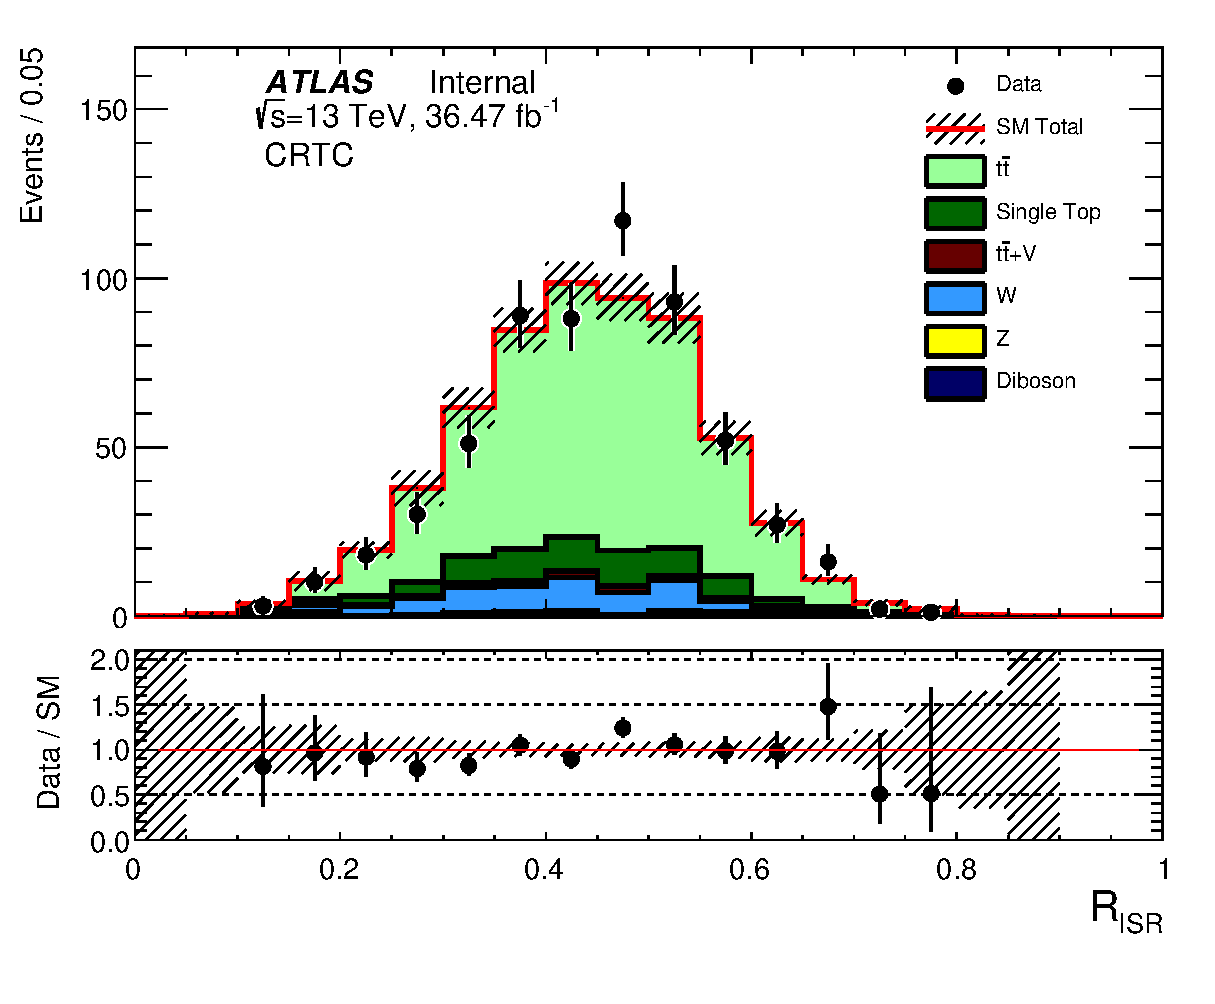
\includegraphics[width=0.45\textwidth]{figures/ttbar/postfit/CA_RISR_CRTopC}
    \includegraphics[width=0.45\textwidth]{figures/ttbar/postfit/CA_pTISR_CRTopC}
    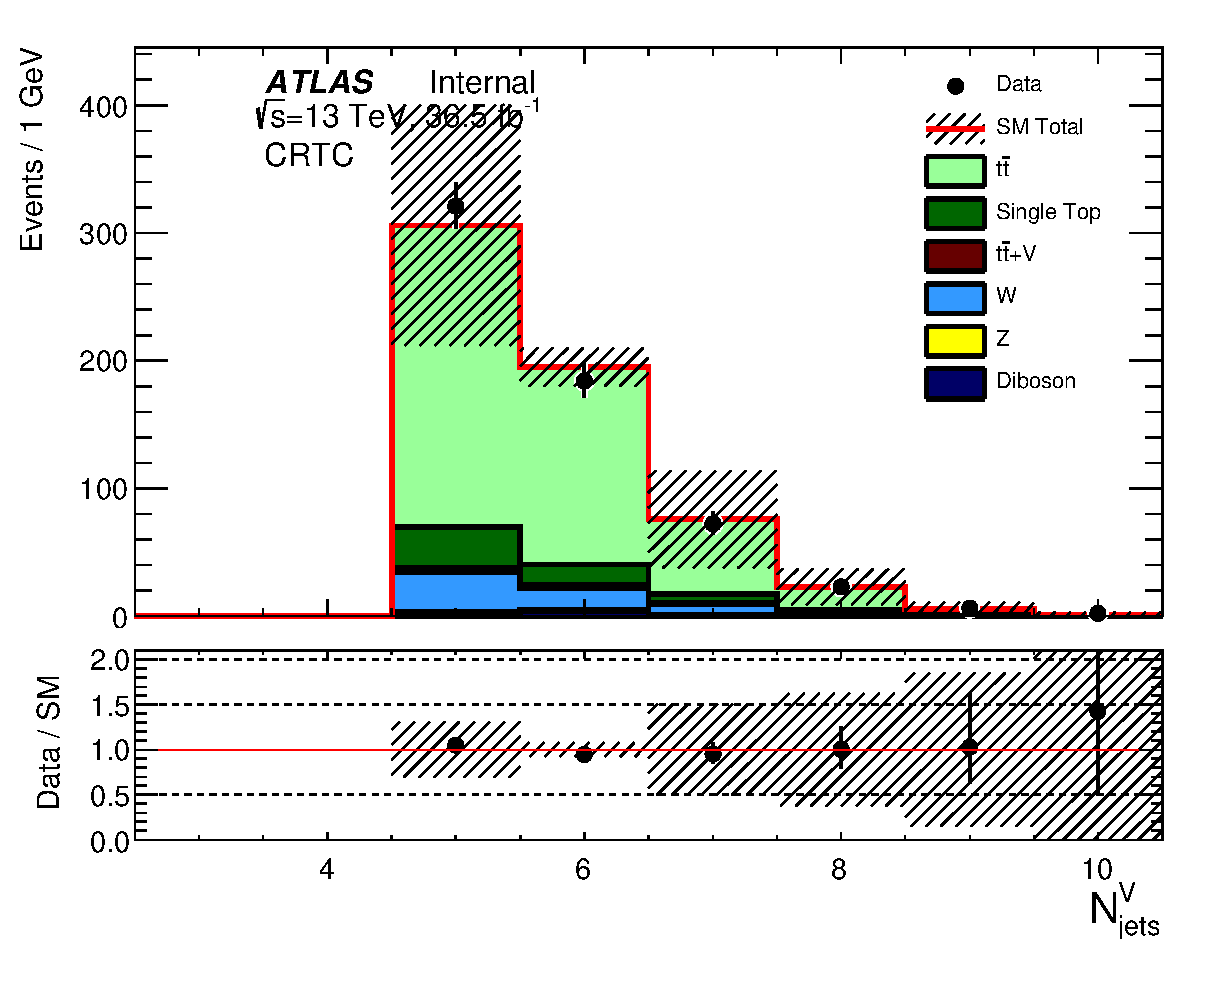
\includegraphics[width=0.45\textwidth]{figures/ttbar/postfit/CA_NjV_CRTopC}
    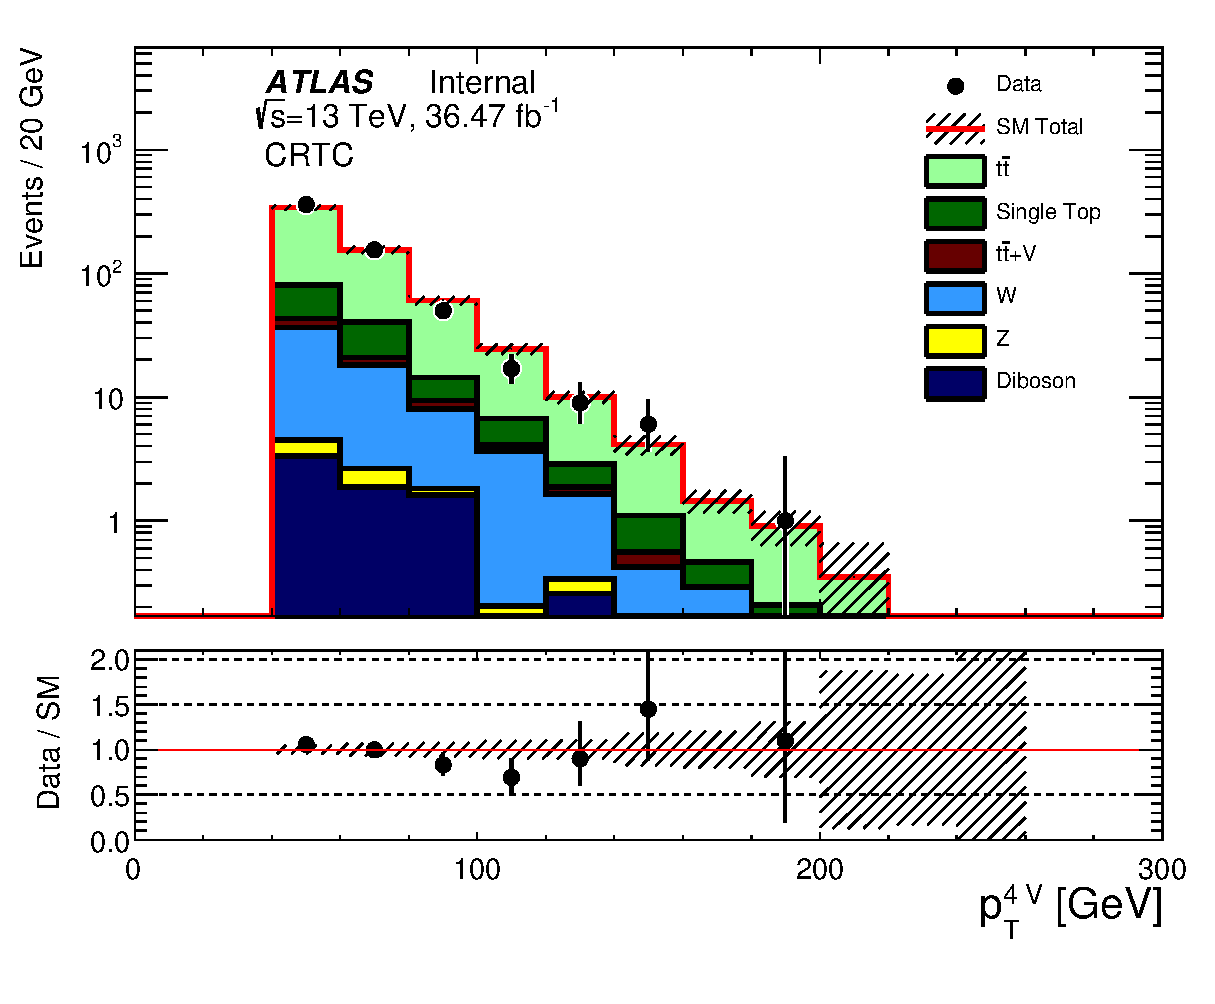
\includegraphics[width=0.45\textwidth]{figures/ttbar/postfit/CA_pTjV4_CRTopC_log}
    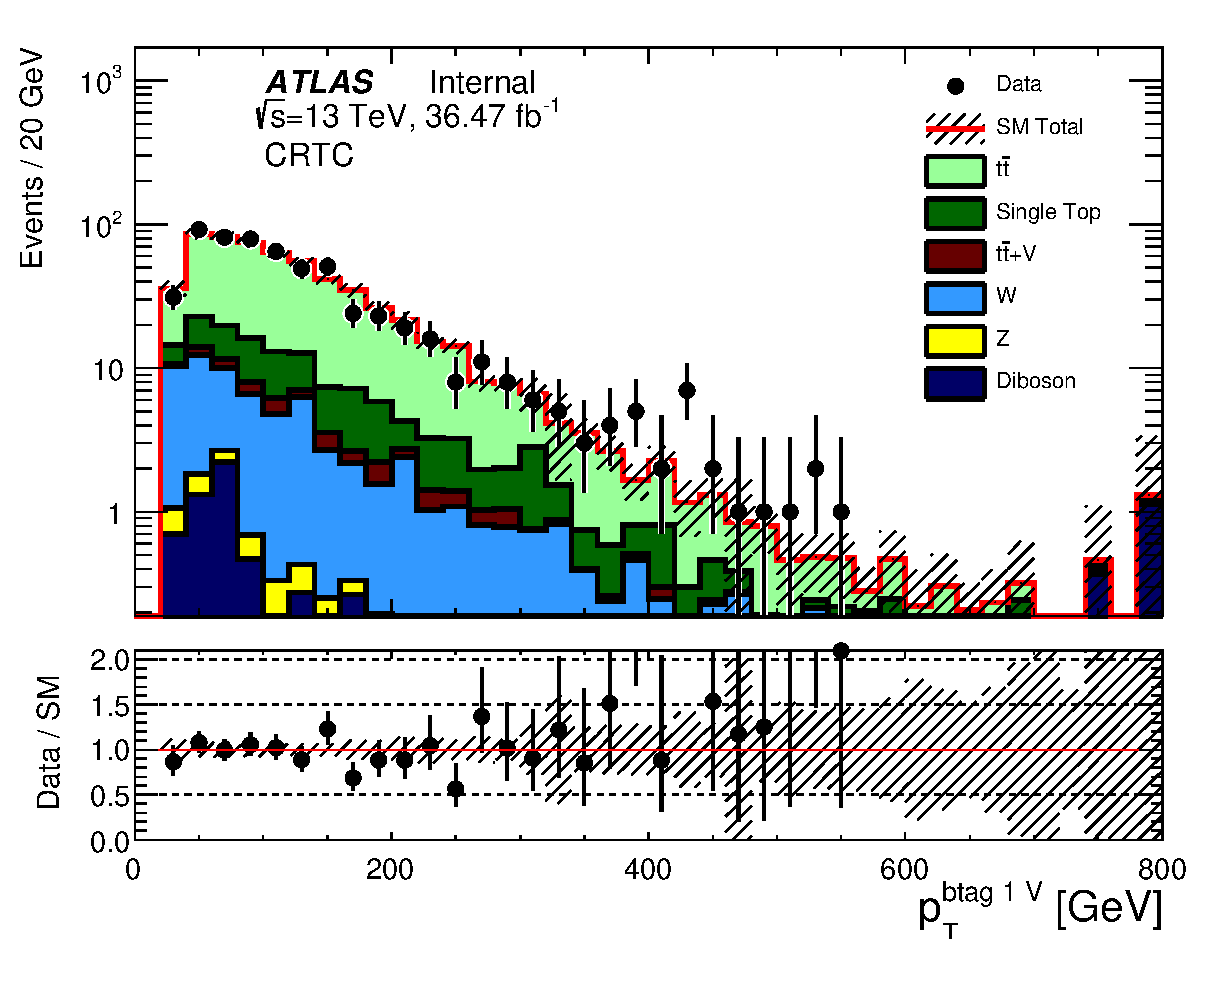
\includegraphics[width=0.45\textwidth]{figures/ttbar/postfit/CA_pTbV1_CRTopC_log}
  \end{center}
  \caption{{\bf NEEDS PLOTS} Distributions for signal region selection. The ratio between data and MC is shown in the bottom panel. The hashed area in both the top and lower panel represent the uncertainty due to MC statistics and detector plus theoretical systematic uncertainties}
  \label{fig:SR}
\end{figure}

\section{Signal Region Background Composition}
\label{sec:Bkg:Compositiion}

The dominate background in all signal region bins is standard model pair produced tops (t\tbar).  The breakdown of background composition is given in table \ref{tab:SRBkg} 

\begin{table}[htpb]
  \caption{Standard Model Background Composition in the Signal Region ~\ref{tab:SRBkg}. }
  \begin{center}
    \def\arraystretch{1.4}%
    \begin{tabular}{c||c|c|c|c|c|c|} \hline\hline
      \RISR Range & 0.20-0.30 & 0.30-0.40 & 0.40-0.50 & 0.50-0.60 & 0.60-0.70 & 0.70-0.80\\  \hline
      t\tbar  &  & & & & & \\  \hline
      W+jets &  & & & & & \\  \hline 
      Z+jets  &  & & & & & \\  \hline 
      Others (dibosons+Single Top+QCD)  &  & & & & & \\ \hline \hline
    \end{tabular}
  \end{center}
  \label{tab:SignalRegion}
\end{table}%

t\tbar accounts for $85$ percent of all backgrounds in the signal region.  The next most prevalent background is W+jets which can reach up to 15 percent in high \RISR\ bins.
